\section{Initial Experiment: Intelligent Algorithm on Small Data}

\subsection{Dataset Description and Preliminary EDA}

This initial experiment utilizes a small, real-world pilot dataset from \textbf{25 patients} to test the feasibility of predicting lung cancer biomarkers (TTF1 and NAPSIN) from 3D CT scans and associated radiomics data.

\subsubsection{Data Source}
The dataset is multi-modal, composed of:
\begin{itemize}
    \item \textbf{\texttt{PatientsData.csv}:} A metadata file containing patient identifiers (\texttt{Code}) and a \texttt{Biopsy positive} column, which serves as the ground truth for our target labels.
    \item \textbf{Raw 3D CT Scans:} Volumetric CT scans in \texttt{.nii.gz} format.
    \item \textbf{Raw 3D PET Scans:} Volumetric PET scans (also \texttt{.nii.gz}).
    \item \textbf{Radiomics Features:} 107 pre-extracted radiomics features in \texttt{.txt} files for each patient.
\end{itemize}

\subsubsection{Initial Data Processing Pipeline}
An initial preprocessing pipeline (\texttt{imageFormat.ipynb}, \texttt{imagePreprocess.ipynb}) was established to standardize this heterogeneous data for a proof-of-concept model:

\begin{itemize}
    \item \textbf{Lung Segmentation:} The \texttt{lungmask} library was used on the raw CT scans to generate binary lung masks (\texttt{.nrrd} files). This isolates the lungs as the primary region of interest.
    \item \textbf{Label Extraction:} The \texttt{Biopsy positive} column was parsed (\texttt{initalModel.ipynb}, cell 4) to create two binary target labels: \textbf{\texttt{TTF1}} (positive/negative) and \textbf{\texttt{NAPSIN}} (positive/negative).
    \item \textbf{CT Volume Processing:}
    \begin{enumerate}
        \item \textbf{Resampling:} CT scans and masks were resampled to a uniform spacing of \textbf{(1.0, 1.0, 3.8) mm}.
        \item \textbf{Masking:} Voxels outside the resampled lung mask were set to \textbf{-1000 HU}.
        \item \textbf{Cropping:} The masked CT was cropped to the lung's bounding box plus a \textbf{5mm margin}.
        \item \textbf{Normalization:} Intensities were clipped to \textbf{[-1000 HU, 400 HU]} and then min-max normalized to \textbf{[0, 1]}.
        \item \textbf{Final Resizing:} The resulting volume was resized via 3D interpolation to a fixed shape of \textbf{(128, 128, 128)} to serve as the 3D CNN input.
    \end{enumerate}
    \item \textbf{Radiomics Feature Processing:} The 107 radiomics features were standardized using \texttt{sklearn.preprocessing.StandardScaler}. The scaler was fit \textit{only} on the training set.
\end{itemize}

\subsubsection{Preliminary EDA}
The final processed dataset consists of 25 samples.
\begin{itemize}
    \item \textbf{Label Distribution (Ground Truth):}
    \begin{itemize}
        \item \textbf{TTF1:} 13 positive (1) / 12 negative (0)
        \item \textbf{NAPSIN:} 11 positive (1) / 14 negative (0)
    \end{itemize}
    \item \textbf{Model Inputs (per patient):}
    \begin{enumerate}
        \item \textbf{3D CT Volume:} Tensor of shape \texttt{(128, 128, 128, 1)}.
        \item \textbf{Radiomics Vector:} Feature vector of shape \texttt{(107)}.
    \end{enumerate}
\end{itemize}

\subsubsection{Ethical Considerations}
As this experiment uses real patient data, all information has been anonymized using a non-identifiable \texttt{Code} to ensure privacy.

\subsection{Intelligent Algorithm}

\subsubsection{Algorithm Choice}
For this first attempt, we hypothesized that a standard 3D CNN would likely fail given the extremely small dataset. Therefore, we proposed a \textbf{multi-modal, dual-input deep learning model} combining:
\begin{enumerate}
    \item A \textbf{3D Convolutional Neural Network (3D CNN)} for spatial feature extraction from CT volumes.
    \item A \textbf{Multi-Layer Perceptron (MLP)} for pattern recognition in the tabular radiomics data.
\end{enumerate}

\subsubsection{Motivation}
The goal of this architecture was to test if \textbf{fusing} low-level, learned spatial features (CNN) with high-level, engineered features (MLP) could provide a detectable predictive signal, even with a minimal dataset. We also employ a \textbf{multi-task learning} approach, with a shared body and two separate output heads, to allow the model to learn a common representation for both TTF1 and NAPSIN prediction.

\subsubsection{Initial Baseline Architecture (\texttt{build\_multimodal\_twoheads})}
The model was implemented in \texttt{TensorFlow/Keras}.
\begin{itemize}
    \item \textbf{CT Branch (3D CNN):}
    \begin{itemize}
        \item \textbf{Input:} \texttt{(128, 128, 128, 1)}
        \item \textbf{Body:} A stack of 3D convolutional blocks (Conv3D $\rightarrow$ BatchNormalization $\rightarrow$ ReLU) and 3D Max Pooling, with filter depth increasing (16 $\rightarrow$ 32 $\rightarrow$ 64 $\rightarrow$ 128).
        \item \textbf{Head:} GlobalAveragePooling3D followed by Dropout (0.3) to produce a 128-dim vector.
    \end{itemize}
    \item \textbf{Radiomics Branch (MLP):}
    \begin{itemize}
        \item \textbf{Input:} \texttt{(107)}
        \item \textbf{Body:} Dense(256, 'relu') $\rightarrow$ Dropout(0.3) $\rightarrow$ Dense(128, 'relu').
    \end{itemize}
    \item \textbf{Fusion:} The 128-dim CT vector and 128-dim radiomics vector are concatenated.
    \item \textbf{Shared Head:} A shared Dense(128, 'relu') layer with Dropout (0.3).
    \item \textbf{Multi-Task Outputs:} Two independent output heads:
    \begin{itemize}
        \item \textbf{TTF1 Head:} \texttt{Dense(1, activation='sigmoid')}
        \item \textbf{NAPSIN Head:} \texttt{Dense(1, activation='sigmoid')}
    \end{itemize}
\end{itemize}



\subsubsection{Libraries Used}
\begin{itemize}
    \item \textbf{Data Handling:} \texttt{pandas}, \texttt{numpy}, \texttt{nibabel}, \texttt{SimpleITK}, \texttt{scipy}
    \item \textbf{Deep Learning:} \texttt{tensorflow}, \texttt{keras}
    \item \textbf{Preprocessing:} \texttt{scikit-learn}, \texttt{lungmask}
\end{itemize}

\subsection{Experimental Methodology and Preliminary Results}

\subsubsection{Data Split}
The small cohort (n=25) was explicitly split by \texttt{Code} to prevent data leakage. This resulted in an \textbf{extremely small training set (n=10)}, which is the primary limitation of this initial experiment.
\begin{itemize}
    \item \textbf{Training Set:} 10 patients
    \item \textbf{Validation Set:} 7 patients
    \item \textbf{Test Set:} 8 patients
\end{itemize}

\subsubsection{Training and Hyperparameters}
\begin{itemize}
    \item \textbf{Optimizer:} Adam (Learning Rate: 1e-4)
    \item \textbf{Callbacks:} \texttt{ReduceLROnPlateau} (patience=3) and \texttt{EarlyStopping} (patience=8, monitoring \texttt{val\_loss}).
    \item \textbf{Loss Function:} \texttt{binary\_crossentropy} (summed for both tasks).
    \item \textbf{Epochs:} 100 (stopped early by callback)
    \item \textbf{Batch Size:} 2
\end{itemize}

\subsubsection{Evaluation Metrics}
The model was evaluated on the 8-patient test set using a \textbf{prediction threshold of 0.40}. Metrics include Accuracy, Precision, Recall, F1-Score, and the Confusion Matrix.

\subsubsection{Preliminary Results}
The results on the test set are presented as a baseline for this first attempt.

\textbf{TTF1 (Test Set, Threshold=0.40):}
\begin{itemize}
    \item \textbf{Accuracy:} 0.5714
    \item \textbf{Precision:} 0.5000
    \item \textbf{Recall:} 0.6667
    \item \textbf{F1-Score:} 0.5714
\end{itemize}

\begin{figure}[h]
    \centering
    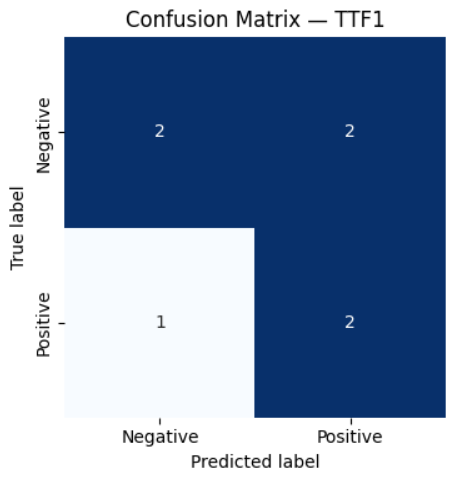
\includegraphics[width=0.45\textwidth]{TTF1_confusion_matrix.png}
    \caption{TTF1 Confusion Matrix (Test Set)}
\end{figure}

\textbf{NAPSIN (Test Set, Threshold=0.40):}
\begin{itemize}
    \item \textbf{Accuracy:} 0.7143
    \item \textbf{Precision:} 1.0000
    \item \textbf{Recall:} 0.3333
    \item \textbf{F1-Score:} 0.5000
\end{itemize}

\begin{figure}[h]
    \centering
    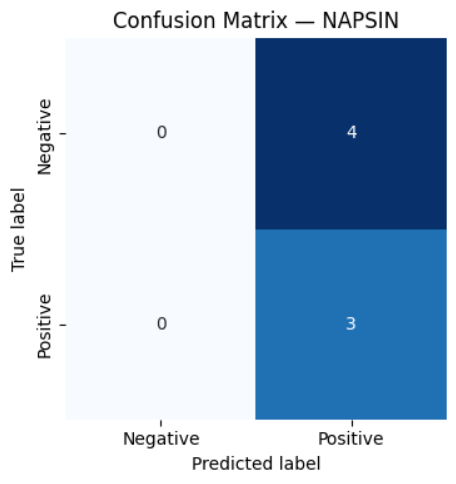
\includegraphics[width=0.45\textwidth]{NAPSIN_confusion_matrix.png}
    \caption{NAPSIN Confusion Matrix (Test Set)}
\end{figure}

\textbf{Example Predictions (Raw Sigmoid Outputs):}
\begin{verbatim}
TTF1: [0.386, 0.429, 0.443, 0.464, 0.607]
NAPSIN: [0.538, 0.530, 0.473, 0.549, 0.578]
\end{verbatim}

\subsubsection{Analysis of First Attempt}
As expected given the extremely limited training data (n=10), the model's performance is not clinically viable but serves as an important proof-of-concept. 

The NAPSIN model showed a tendency to learn the majority negative class, resulting in perfect precision (it was correct when it predicted positive) but very poor recall (it missed 2 of the 3 positive cases). The TTF1 model's performance (57.1\% accuracy) was only slightly better than random chance.

This experiment successfully establishes a full processing and modeling pipeline. The results, while modest, confirm that the model is learning \textit{some} signal (outperforming random chance, especially on NAPSIN precision). This outcome justifies the hypothesis that a multi-modal approach is necessary and strongly indicates that further investigation with a significantly larger dataset is warranted to train a generalizable model.